\documentclass[style=paintings]{powerdot}

\usepackage{graphicx}

\title{\TeX tacular}
\author{Trevor Maglione}
\date{11 March 2014}

\begin{document}
\maketitle
\begin{slide}{Overview}
  \twocolumn{
    \subsection*{Idea}
    \begin{itemize}
    \item Make \LaTeX\ accessible to everyone
    \item Simplify creation of beautiful documents
    \end{itemize}
  }{
    \subsection*{Audience}
    \begin{itemize}
    \item Users who prefer point-and-click and simple forms over
      manual creation of \TeX\ source
    \item Those less technically inclined
    \end{itemize}
  }
\end{slide}
\begin{slide}{Implementation}
  \twocolumn{
    \begin{figure}
      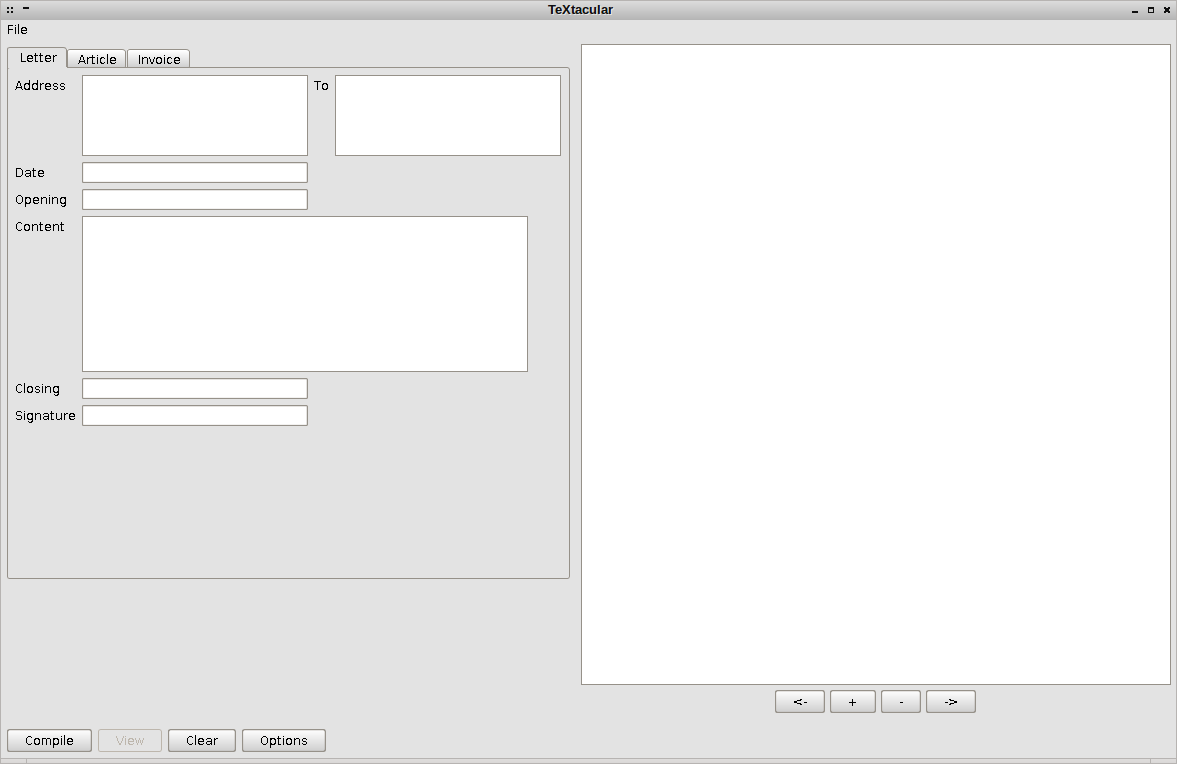
\includegraphics[width=0.9\textwidth]{screens/one.eps}
      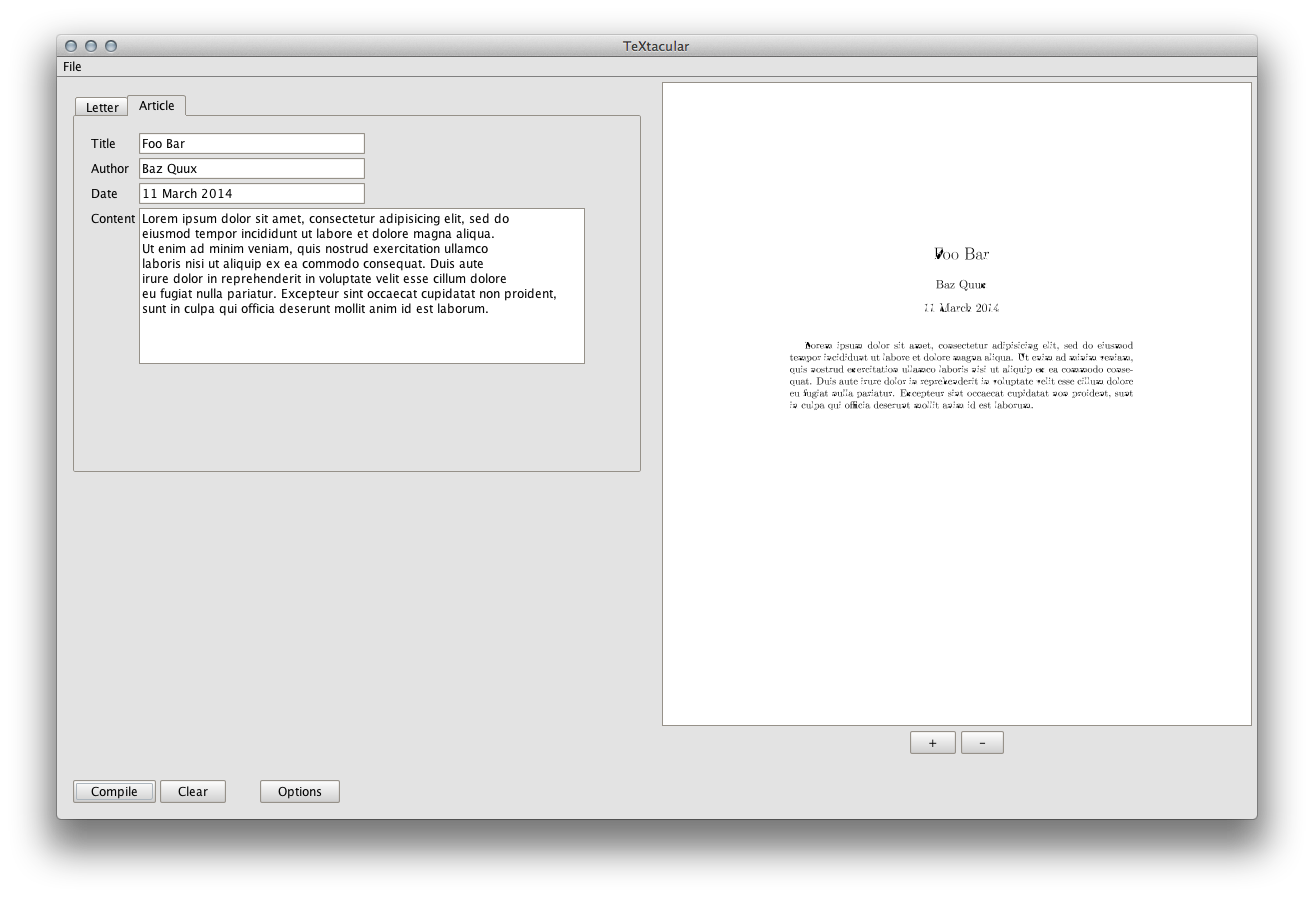
\includegraphics[width=0.9\textwidth]{screens/two.eps}
    \end{figure}
  }{
    \subsection*{Implementation Details}
    \begin{itemize}
      \item Main frame contains a concrete \texttt{TemplatePanel} with
        inputs, a few buttons at the bottom, and a
        \texttt{PreviewPanel} on the right
      \item A \texttt{TeXHandler} class handles compilation of \TeX\
        source
        \begin{itemize}
          \item Uses \texttt{latexmk} and a script to compile
        \end{itemize}
      \item \texttt{PreviewPanel} updates automatically with the
        contents of the compiled PDF
      \item Third party libraries
        \begin{itemize}
          \item MiGLayout
          \item Sun PDF-Renderer
          \item PgsLookAndFeel
        \end{itemize}
    \end{itemize}
  }
\end{slide}
\begin{slide}{Notes}
  \twocolumn{
    \subsection*{Difficulties \& Concerns}
    \begin{itemize}
      \item How best to handle template types
      \item Reasonable method of laying out components without a
        completely different strategy for each template type
      \item Auto-updating PDF panel and zooming (conversion of PDF to a
        \texttt{BufferedImage} -- far from perfect
      \item Handling application and \texttt{latexmk} compilation errors
    \end{itemize}
  }{
    \subsection*{Future}
    \begin{itemize}
      \item Improve scrolling inside preview panel
        \begin{itemize}
          \item Currently click and drag but can be flaky
        \end{itemize}
      \item More general, approachable way for building templates
      \item Improve scaling of PDF preview
      \item Add ``Save'', ``Load'', ``Print'' options
      \item Add Windows support
    \end{itemize}
  }
\end{slide}
\end{document}
